\documentclass[a4paper, 12pt]{article}
\usepackage[utf8]{inputenc}
\usepackage[english, ukrainian]{babel}

\usepackage{amsmath, amssymb}
\usepackage{multicol}
\usepackage{graphicx}
\usepackage{float}

\allowdisplaybreaks
\setlength\parindent{0pt}
\numberwithin{equation}{subsection}

\usepackage{hyperref}
\hypersetup{unicode=true,colorlinks=true,linktoc=all,linkcolor=red}

\numberwithin{equation}{subsection}

\renewcommand{\bf}[1]{\textbf{#1}}
\renewcommand{\it}[1]{\textit{#1}}
\newcommand{\bb}[1]{\mathbb{#1}}
\renewcommand{\cal}[1]{\mathcal{#1}}

\renewcommand{\epsilon}{\varepsilon}
\renewcommand{\phi}{\varphi}

\DeclareMathOperator{\diam}{diam}
\DeclareMathOperator{\rang}{rang}
\DeclareMathOperator{\const}{const}

\newenvironment{system}{%
  \begin{equation}%
    \left\{%
      \begin{aligned}%
}{%
      \end{aligned}%
    \right.%
  \end{equation}%
}
\newenvironment{system*}{%
  \begin{equation*}%
    \left\{%
      \begin{aligned}%
}{%
      \end{aligned}%
    \right.%
  \end{equation*}%
}

\makeatletter
\newcommand*{\relrelbarsep}{.386ex}
\newcommand*{\relrelbar}{%
  \mathrel{%
    \mathpalette\@relrelbar\relrelbarsep%
  }%
}
\newcommand*{\@relrelbar}[2]{%
  \raise#2\hbox to 0pt{$\m@th#1\relbar$\hss}%
  \lower#2\hbox{$\m@th#1\relbar$}%
}
\providecommand*{\rightrightarrowsfill@}{%
  \arrowfill@\relrelbar\relrelbar\rightrightarrows%
}
\providecommand*{\leftleftarrowsfill@}{%
  \arrowfill@\leftleftarrows\relrelbar\relrelbar%
}
\providecommand*{\xrightrightarrows}[2][]{%
  \ext@arrow 0359\rightrightarrowsfill@{#1}{#2}%
}
\providecommand*{\xleftleftarrows}[2][]{%
  \ext@arrow 3095\leftleftarrowsfill@{#1}{#2}%
}
\makeatother

\newcommand{\NN}{\mathbb{N}}
\newcommand{\ZZ}{\mathbb{Z}}
\newcommand{\QQ}{\mathbb{Q}}
\newcommand{\RR}{\mathbb{R}}
\newcommand{\CC}{\mathbb{C}}

\newcommand{\Max}{\displaystyle\max\limits}
\newcommand{\Sup}{\displaystyle\sup\limits}
\newcommand{\Sum}{\displaystyle\sum\limits}
\newcommand{\Int}{\displaystyle\int\limits}
\newcommand{\Iint}{\displaystyle\iint\limits}
\newcommand{\Lim}{\displaystyle\lim\limits}

\newcommand*\diff{\mathop{}\!\mathrm{d}}

\newcommand*\rfrac[2]{{}^{#1}\!/_{\!#2}}


\title{{\Huge МАТЕМАТИЧНА ФІЗИКА}}
\author{Скибицький Нікіта}
\date{\today}

\usepackage{amsthm}
\usepackage[dvipsnames]{xcolor}
\usepackage{thmtools}
\usepackage[framemethod=TikZ]{mdframed}

\theoremstyle{definition}
\mdfdefinestyle{mdbluebox}{%
	roundcorner = 10pt,
	linewidth=1pt,
	skipabove=12pt,
	innerbottommargin=9pt,
	skipbelow=2pt,
	nobreak=true,
	linecolor=blue,
	backgroundcolor=TealBlue!5,
}
\declaretheoremstyle[
	headfont=\sffamily\bfseries\color{MidnightBlue},
	mdframed={style=mdbluebox},
	headpunct={\\[3pt]},
	postheadspace={0pt}
]{thmbluebox}

\mdfdefinestyle{mdredbox}{%
	linewidth=0.5pt,
	skipabove=12pt,
	frametitleaboveskip=5pt,
	frametitlebelowskip=0pt,
	skipbelow=2pt,
	frametitlefont=\bfseries,
	innertopmargin=4pt,
	innerbottommargin=8pt,
	nobreak=true,
	linecolor=RawSienna,
	backgroundcolor=Salmon!5,
}
\declaretheoremstyle[
	headfont=\bfseries\color{RawSienna},
	mdframed={style=mdredbox},
	headpunct={\\[3pt]},
	postheadspace={0pt},
]{thmredbox}

\declaretheorem[style=thmbluebox,name=Теорема,numberwithin=subsubsection]{theorem}
\declaretheorem[style=thmbluebox,name=Лема,numberwithin=subsubsection]{lemma}
\declaretheorem[style=thmbluebox,name=Твердження,numberwithin=subsubsection]{proposition}
\declaretheorem[style=thmbluebox,name=Принцип,numberwithin=subsubsection]{th_principle}
\declaretheorem[style=thmbluebox,name=Закон,numberwithin=subsubsection]{law}
\declaretheorem[style=thmbluebox,name=Закон,numbered=no]{law*}
\declaretheorem[style=thmbluebox,name=Формула,numberwithin=subsubsection]{th_formula}
\declaretheorem[style=thmbluebox,name=Рівняння,numberwithin=subsubsection]{th_equation}
\declaretheorem[style=thmbluebox,name=Умова,numberwithin=subsubsection]{th_condition}
\declaretheorem[style=thmbluebox,name=Наслідок,numberwithin=subsubsection]{corollary}

\declaretheorem[style=thmredbox,name=Приклад,numberwithin=subsubsection]{example}
\declaretheorem[style=thmredbox,name=Приклади,sibling=example]{examples}

\declaretheorem[style=thmredbox,name=Властивість,numberwithin=subsubsection]{property}
\declaretheorem[style=thmredbox,name=Властивості,sibling=property]{properties}

\mdfdefinestyle{mdgreenbox}{%
	skipabove=8pt,
	linewidth=2pt,
	rightline=false,
	leftline=true,
	topline=false,
	bottomline=false,
	linecolor=ForestGreen,
	backgroundcolor=ForestGreen!5,
}
\declaretheoremstyle[
	headfont=\bfseries\sffamily\color{ForestGreen!70!black},
	bodyfont=\normalfont,
	spaceabove=2pt,
	spacebelow=1pt,
	mdframed={style=mdgreenbox},
	headpunct={ --- },
]{thmgreenbox}

\mdfdefinestyle{mdblackbox}{%
	skipabove=8pt,
	linewidth=3pt,
	rightline=false,
	leftline=true,
	topline=false,
	bottomline=false,
	linecolor=black,
	backgroundcolor=RedViolet!5!gray!5,
}
\declaretheoremstyle[
	headfont=\bfseries,
	bodyfont=\normalfont\small,
	spaceabove=0pt,
	spacebelow=0pt,
	mdframed={style=mdblackbox}
]{thmblackbox}

\declaretheorem[name=Вправа,numberwithin=subsubsection,style=thmblackbox]{exercise}
\declaretheorem[name=Зауваження,numberwithin=subsubsection,style=thmgreenbox]{remark}
\declaretheorem[name=Визначення,numberwithin=subsubsection,style=thmblackbox]{definition}

\newtheorem{problem}{Задача}[subsection]
\newtheorem{sproblem}[problem]{Задача}
\newtheorem{dproblem}[problem]{Задача}
\renewcommand{\thesproblem}{\theproblem$^{\star}$}
\renewcommand{\thedproblem}{\theproblem$^{\dagger}$}
\newcommand{\listhack}{$\empty$\vspace{-2em}} 

\theoremstyle{remark}
\newtheorem*{solution}{Розв'язок}


\begin{document}

\tableofcontents

\setcounter{section}{4}
\setcounter{subsection}{3}
\setcounter{subsubsection}{4}
\setcounter{theorem}{21}
\setcounter{equation}{55}

\subsubsection{Функція Гріна граничних задач оператора теплопровідності}

Будемо розглядати граничні задачі для рівняння теплопровідності:

\begin{system}
	& a^2 \Delta u(x, t) - \frac{\partial u(x,t)}{\partial t} = - F(x, t), \\
	& u(x, 0) = u_0(x), \\
	& \left. \ell_i u(x, t) \right|_{x \in S} = f(x, t), \quad i = 1, 2, 3.
\end{system}
для $x \in \Omega$, $t > 0$. \medskip

Тут 
\begin{align}
	\left. \ell_1 u(x, t) \right|_{x \in S} &= \left. u(x, t) \right|_{x \in S}, \\
	\left. \ell_2 u(x, t) \right|_{x \in S} &= \left. \frac{\partial u(x, t)}{\partial n} \right|_{x \in S}, \\
	\left. \ell_3 u(x, t) \right|_{x \in S} &= \left. \frac{\partial u(x, t)}{\partial n} + \alpha(x, t) \cdot u(x, t) \right|_{x \in S}
\end{align}
--- оператори граничних умов першого, другого, або третього роду.

\begin{definition}[функції Гріна рівняння теплопровідності]
	Функцію $E_i (x, \xi, t - \tau)$ будемо називати \textit{функцією Гріна першої, другої або третьої граничної задачі рівняння теплопровідності} в області $\Omega$ з границею $S$ для $t > 0$, якщо вона є розв'язком настуної граничної задачі:
	\begin{system}
		& a^2 \Delta_x E_i (x, \xi, t - \tau) - \frac{\partial E_i(x, \xi, t - \tau)}{\partial t} = - \delta(x - \xi, t - \tau), \\
		& \left. E_i(x, \xi, t - \tau) \right|_{t - \tau \le 0} = 0, \\
		& \left. \ell_i E_i (x, \xi, t - \tau) \right|_{x \in S} = 0, \quad i = 1, 2, 3.
	\end{system}
	для $x \in \Omega$, $t > 0$
\end{definition}

Еквівалетнне визначення можна надати у вигляді
\begin{definition}[функції Гріна рівняння теплопровідності]
	Функцію $E_i (x, \xi, t - \tau)$ будемо називати \textit{функцією Гріна першої, другої або третьої граничної задачі рівняння теплопровідності} в області $\Omega$ з границею $S$ для $t > 0$, якщо вона може бути представлена у вигляді
	\begin{equation}
		E_i(x, \xi, t - \tau) = \epsilon(x - \xi, t - \tau) + \omega_i(x, \xi, t - \tau),
	\end{equation}
	де  перший доданок є фундаментальним розв'язком оператора теплопровідності, а другий  є розв'язком наступної граничної задачі
	\begin{system}
		& a^2 \Delta_x \omega_i (x, \xi, t - \tau) - \frac{\partial \omega_i(x, \xi, t - \tau)}{\partial t} = - \delta(x - \xi, t - \tau), \\
		& \left. \omega_i(x, \xi, t - \tau) \right|_{t - \tau \le 0} = 0, \\
		& \left. \ell_i \omega_i (x, \xi, t - \tau) \right|_{x \in S} = -\left.\ell_i \epsilon_i(x - \xi, t - \tau)\right|_{x \in S} \quad i = 1, 2, 3.
	\end{system}
	для $x \in \Omega$, $t > 0$.
\end{definition}

Вивчимо 
\begin{properties}[функції Гріна оператора теплопровідності]
	Легко бачити, що 
	\begin{enumerate}
		\item Функція Гріна граничних задач рівняння теплопровідності з аргументами $E_i(x, \xi, -t)$ задовольняє спряженому диференціальному рівнянню
		\begin{equation}
			a^2 \Delta_x E_i(x, \xi, -t) + \frac{\partial E_i(x, \xi, - t)}{\partial t} = - \delta(x - \xi) \delta (t - \tau), 
		\end{equation}
		для усіх $x, \xi \in \Omega$, і $t > 0$.
		\item Функція Гріна є також симетричною функцією своїх перших двох аргументів.
	\end{enumerate}
\end{properties}
	
\begin{proof}
	Доведемо другу властивість. Запишемо співвідношення, яким задовольняє функція Гріна:
	\begin{align}
		a^2 \Delta_x E_i(x, \xi, t - \tau_1) + \frac{\partial E_i(x, \xi, t - \tau_1)}{\partial t} &= - \delta(x - \xi) \delta (t - \tau_1), \quad x, \xi \in \Omega, \\
		a^2 \Delta_x E_i(x, \eta, \tau_2 - t) + \frac{\partial E_i(x, \eta, \tau_2 - t)}{\partial t} &= - \delta(x - \eta) \delta (t - \tau_2), \quad x, \eta \in \Omega.
	\end{align}
	Перше рівняння помножимо на $E_i(x, \xi, \tau_2 - t)$, друге рівняння помножимо на $E_i(x, \xi, t - \tau_1)$, віднімемо від першого друге і проінтегруємо по $x \in \Omega$ і по $-\infty < t < \tau$:
	\begin{equation}
		\begin{aligned}
			& a^2 \Iiint_\Omega \Int_{-\infty}^\tau \Big( E_i(x, \eta, \tau_2 - t) \Delta_x E_i(x, \xi, t - \tau_1) - \\
			& \qquad \quad - E_i(x, \xi, t - \tau_1) \Delta_x E_i(x, \eta, \tau_2 - t) \Big) \diff t \diff x - \\
			& \qquad - \Iiint_\Omega \Int_{-\infty}^\tau \frac{\partial}{\partial \tau} \left( E_i(x, \xi, t - \tau_1) E_i(x, \eta, \tau_2 - t) \right) \diff t \diff x = \\
			& \quad = - E_i(\xi, \eta, \tau_2 - \tau_1) + E_i(\eta, \xi, \tau_2 - \tau_1).
		\end{aligned}
	\end{equation}

	В результаті застосування другої формули Гріна до першого інтегралу в лівій частині рівності і обчислення другого інтегралу лівої частини, отримаємо:
	\begin{equation}
		\begin{aligned}
			& E_i(\xi, \eta, \tau_2 - \tau_1 ) - E_i(\eta, \xi, \tau_2 - \tau_1) = \\
			& \quad = - \Iiint_\Omega \Big( E_i(x, \xi, \tau - \tau_1) E_i(x, \eta, \tau_2 - \tau) - \\
			& \qquad \quad - E_i(x, \xi, -\infty) E_i(x, \eta, -\infty) \Big) \diff \Omega + \\
			& \qquad + a^2 \Iint_S \Int_{-\infty}^\tau \left( \frac{\partial E_i(x, \xi, t - \tau_1)}{\partial n} E_i(x, \eta, \tau_2 - t) \right. - \\
			& \qquad \quad - \left. E_i(x, \xi, t - \tau_1) \frac{\partial E_i(x, \eta, \tau_2 - t)}{\partial n} \right) \diff S \diff t.
		\end{aligned}
	\end{equation}

	Обираючи $\tau > \tau_2 > \tau_1$ , отримаємо з урахування граничних і початкових умов для функції Гріна, що інтеграли в правій частині останньої рівності дорівнює нулю.
\end{proof}

Для отримання інтегрального представлення розв'язків граничних задач, запишемо граничну задачу теплопровідності в змінних $\xi$, $\tau$ :
\begin{system}
	& a^2 \Delta u(\xi, \tau) - \frac{\partial u(\xi, \tau)}{\partial \tau} = - F(\xi, \tau), \quad \xi \in \Omega, \quad \tau > 0, \\
	& u(\xi, 0) = u_0(\xi), \\
	& \left. \ell_i u(\xi, \tau) \right|_{\xi \in S} = f(\xi, \tau), \quad i = 1, 2, 3. 
\end{system}
та рівняння для функції Гріна по змінних $\xi$, $\tau$:
\begin{equation}
	a^2 \Delta_\xi E_i(x, \xi, t - \tau) + \frac{\partial E_i(x, \xi, t - \tau)}{\partial \tau} = - \delta(x - \xi) \delta(t - \tau),
\end{equation}
де $x, \xi \in \Omega$, $ t > \tau > 0$. \medskip

Перше рівняння помножимо на $E_i(x, \xi, t - \tau)$, а друге --- на $u(\xi, \tau$, віднімемо від першого друге, і проінтегруємо по $0 < \tau < t + \epsilon$ та по $\xi \in \Omega$. \medskip

Отриаємо співвідношення:
\begin{equation}
	\begin{aligned}
		& a^2 \Int_0^{t + \epsilon} \Iiint_\Omega \Big( E_i(x, \xi, t - \tau) \Delta u(\xi, \tau) - \\
		& \qquad \quad - u(\xi, \tau) \Delta_\xi E_i(x, \xi, t - \tau) \Big) \diff \xi \diff \tau + \\
		& \qquad + \Int_0^{t + \epsilon} \Iiint_\Omega E_i(x, \xi, t - \tau) F(\xi, \tau) \diff \xi \diff \tau - \\
		& \qquad -  \Iiint_\Omega \Int_0^{t+\epsilon} \frac{\partial (E_u(x, \xi, t - \tau) u(\xi, \tau))}{\partial \tau} \diff \tau \diff \xi = \\
		& \quad =  \Int_0^{t + \epsilon} \Iiint_\Omega \delta(x - \xi) \delta(t - \tau) \diff \xi \diff \tau.
	\end{aligned}
\end{equation}

Після застосування другої формули Гріна до першого інтегралу, обчислення третього інтегралу при $\epsilon \to 0$ отримаємо наступну проміжну формулу:
\begin{equation}
	\begin{aligned}
		u(x, t) &= \Int_0^t \Iiint_\Omega E_i(x, \xi, t - \tau) F(\xi, \tau) \diff \xi \diff \tau + \\
		& \quad + \Iiint_\Omega E_i(x, \xi, t) u_0(\xi) \diff \xi + \\
		& \quad + a^2 \Int_0^t \Iint_S \left( E_i(x, \xi, t - \tau) \frac{\partial u(\xi, \tau)}{\partial n_\xi} - u(\xi, \tau) \frac{\partial E_i(x, \xi, t - \tau)}{\partial n_\xi} \right) \diff S_\xi \diff \tau.
	\end{aligned}
\end{equation}

Враховуючи відповідні граничні умови, яким задовольняє розв'язок на границі поверхні $S$ отримаємо для першої граничної задачі:
\begin{equation}
	\begin{aligned}
		u(x, t) &= \Int_0^t \Iiint_\Omega E_1(x, \xi, t - \tau) F(\xi, \tau) \diff \xi \diff \tau + \\
		& \quad + \Iiint_\Omega E_1(x, \xi, t) u_0(\xi) \diff \xi - \\
		& \quad - a^2 \Int_0^t \Iint_S \left( \frac{\partial E_1(x, \xi, t - \tau)}{\partial n_\xi} f(\xi, \tau)\right) \diff S_\xi \diff \tau.
	\end{aligned}
\end{equation}

Для другої та третьої граничних задач отримаємо 
\begin{equation}
	\begin{aligned}
		u(x, t) &= \Int_0^t \Iiint_\Omega E_i(x, \xi, t - \tau) F(\xi, \tau) \diff \xi \diff \tau + \\
		& \quad + \Iiint_\Omega E_i(x, \xi, t) u_0(\xi) \diff \xi + \\
		& \quad + a^2 \Int_0^t \Iint_S E_i(x, \xi, t - \tau) f(\xi, \tau) \diff S_\xi \diff \tau.
	\end{aligned}
\end{equation}

\subsubsection{Функція Гріна граничних задач хвильового оператора}

Будемо розглядати граничні задачі для хвильового рівняння:

\begin{system}
	& a^2 \Delta u(x, t) - \frac{\partial^2 u(x, t)}{\partial t^2} = -F(x, t), \\
	& u(x, 0) = u_0(x), \\
	& \frac{\partial u(x, 0)}{\partial t} = v_0(x), \\
	& \left. \ell_i u(x, t) \right|_{x \in s} = f(x, t), \quad i = 1, 2, 3.
\end{system}

\begin{definition}[функції Гріна хвильового рівняння]
	Функцію $\Theta_i(x, \xi, t - \tau)$ будемо називати функцією Гріна першої, другої або третьої граничної задачі хвильового рівняння в області $\Omega$ з границею $S$ і $t > 0$, якщо вона є розв'язком наступної граничної задачі:
	\begin{system}
		& a^2 \Delta_x \Theta_i(x, \xi, t - \tau) - \frac{\partial^2 \Theta_i(x, \xi, t - \tau)}{\partial t^2} = - \delta(x - \xi) \delta(t - \tau), \\
		& \left. \Theta_i(x, \xi, t - \tau) \right|_{t - \tau \le 0} = 0, \\
		& \left. \frac{\partial \Theta_i(x, \xi, t - \tau)}{\partial t} \right|_{t - \tau \le 0} = 0, \\
		& \left. \ell_i \Theta_i(x, \xi, t - \tau) \right|_{x \in S} = 0, \quad i = 1, 2, 3.
	\end{system}
\end{definition}

Еквівалентне визначення можна надати у вигляді:
\begin{definition}[функції Гріна хвильового рівняння]
	Функцію $\Theta_i(x, \xi, t - \tau)$ будемо називати функцією Гріна першої, другої або третьої граничної задачі хвильового рівняння в області $\Omega$ з границею $S$ і $t > 0$, якщо вона може бути представлена у вигляді
	\begin{equation}
		\Theta_i(x, \xi, t - \tau) = \psi(x - \xi, t - \tau) + \theta_i(x, \xi, t - \tau),
	\end{equation}
	де перший доданок є фундаментальним розв'язком хвильового оператора, а другий є розв'язком наступної граничної задачі:
	\begin{system}
		& a^2 \Delta_x \theta_i(x, \xi, t - \tau) - \frac{\partial^2 \theta_i(x, \xi, t - \tau)}{\partial t^2} = 0, \\
		& \left. \theta_i(x, \xi, t - \tau) \right|_{t - \tau \le 0} = 0, \\
		& \left. \frac{\partial \theta_i(x, \xi, t - \tau)}{\partial t} \right|_{t - \tau \le 0} = 0, \\
		& \left. \ell_i \theta_i(x, \xi, t - \tau) \right|_{x \in S} = - \left. \ell_i \psi_i(x, \xi, t - \tau) \right|_{x \in S}, \quad i = 1, 2, 3.
	\end{system}
\end{definition}

Використовуючи попередні викладки для рівняння теплопровідності, легко встановити, що функція Гріна хвильового рівняння є симетричною функцією перших двох аргументів і по сукупності аргументів $\xi$, $\tau$ задовольняє рівняння:
\begin{equation}
	a^2 \Delta_\xi \Theta_i(x, \xi, t - \tau) - \frac{\partial^2 \Theta_i(x, \xi, t - \tau)}{\partial t^2} = - \delta(x - \xi) \delta(t - \tau).
\end{equation}

Для розв'язку граничних задач хвильового рівняння можна отримати формули інтегрального представлення аналогічні відповідним формулам для рівняння теплопровідності:
\begin{th_formula}
	Розв'язком першої граничної задачі для хвильового рівняння є 
	\begin{equation}
		\begin{aligned}
			u(x, t) &= \Int_0^t \Iiint_\Omega \Theta_1(x, \xi, t - \tau) F(\xi, \tau) \diff \xi \diff \tau + \\
			& \quad + \Iiint_\Omega \Theta_1(x, \xi, t) v_0(\xi), \diff \xi - \\
			& \quad - \Iiint_\Omega \left. \frac{\partial \Theta_1(x, \xi, t - \tau)}{\partial \tau} \right|_{\tau = 0} u(\xi) \diff \xi - \\
			& \quad - a^2 \Int_0^t \Iint_S \left( \frac{\partial \Theta_1(x, \xi, t - \tau)}{\partial n_\xi} f(\xi, \tau) \right) \diff S_\xi \diff \tau.
		\end{aligned}
	\end{equation}
\end{th_formula}

\begin{exercise}
	Отримайте наведену формулу.
\end{exercise}

\begin{th_formula}
	Розв'язком другої і третьої граничних задач для хвильового рівняння є 
	\begin{equation}
		\begin{aligned}
			u(x, t) &= \Int_0^t \Iiint_\Omega \Theta_i(x, \xi, t - \tau) F(\xi, \tau) \diff \xi \diff \tau + \\
			& \quad + \Iiint_\Omega \Theta_i(x, \xi, t) v_0(\xi), \diff \xi - \\
			& \quad - \Iiint_\Omega \left. \frac{\partial \Theta_1(x, \xi, t - \tau)}{\partial \tau} \right|_{\tau = 0} u(\xi) \diff \xi - \\
			& \quad - a^2 \Int_0^t \Iint_S \Big( \Theta_i(x, \xi, t - \tau) f(\xi, \tau) \Big) \diff S_\xi \diff \tau.
		\end{aligned}
	\end{equation}
\end{th_formula}

\begin{exercise}
	Отримайте наведену формулу.
\end{exercise}

\subsection{Методи побудови функції Гріна для канонічних областей}

Знаходження розв'язку граничної задачі за допомогою функції Гріна для відповідного оператора, заданої області та типу граничних умов фактично зводиться до необхідності розв'язання граничної задачі еквівалентної вихідній з спеціальними граничними умовами. Побудова функції Гріна для довільних областей є задачею такого ж рівня складності як і безпосереднє знаходження розв'язку, в той же час існують так звані канонічні області для яких можна в явному вигляді записати функцію Гріна, а значить побудувати розв'язок граничної задачі. \medskip

До канонічних областей будемо відносити паралелепіпед в прямокутній системі координат, а також області які в ортогональних криволінійних координатах є паралелепіпедами. Зокрема, півпростір, четверта частина простору, двогранний кут величини $\pi / n$, шар, що міститься між двома паралельними площинами, куля та її канонічні частини, циліндр прямокутного та кругового перерізу, паралелепіпед та інші.

\subsubsection{Побудова функції Гріна методом відображення зарядів для граничних задач оператора Лапласа}

Для побудови функції Гріна оператора Лапласа використовується фізична інтерпретація фундаментального розв'язку тривимірного та двовимірного евклідового простору. Нагадаємо, що фундаментальний розв'язок оператора Лапласа має вигляд:
\begin{equation}
	q_0(x) = \begin{cases}
		\dfrac{1}{4 \pi |x|}, & x \in \RR^3, \\
		\dfrac{1}{2 \pi} \ln \dfrac{1}{|x|}, & x \in \RR^2.
	\end{cases}
\end{equation}

Для тривимірного простору фізичний зміст фундаментально розв'язку нам відомий і представляє потенціал електростатичного поля в точці $x$ одиничного точкового заряду, який розташований в початку координат. Для двовимірного випадку ми визначимо фізичний зміст фундаментального розв'язку трохи нижче. \medskip

Таким чином функцію Гріна для деякої просторової області можна шукати у вигляді потенціалу електростатичного поля сукупності точкових або розподілених зарядів, один з яких є одиничним позитивним і знаходиться в довільній внутрішній точці області $\Omega$, а усі інші лежать поза областюю $\Omega$, місце розташування і величина зарядів підбираються таким чином, щоби задовільними однорідним граничним умовам на поверхні області. \medskip

Тобто функція Гріна для канонічних областей дуже часто може бути знайдена у вигляді:
\begin{equation}
	G_i(p, P_0) = \frac{1}{4 \pi |P - P_0|} + \Sum_j \frac{\gamma_j}{4 \pi |P - P_j|}.
\end{equation}

У цый формулі перший доданок є фундаментальним розв'язком і одночасно моделює потенціал в точці $P$ одиничного точкового заряду розташованого в точці $P_0 \in \Omega$. Сума --- другий регулярний доданок, який фігурує в означенні 2 функції Гріна представляє функцію  $g_i^k(x, \xi)$, $\gamma_k$ --- константи, які моделюють величину точкового заряду, $P_j \notin \Omega$ --- точки розташування зарядів, які лежать поза областю $\Omega$. \medskip

Оскільки має місце рівність
\begin{equation}
	\Delta_P \frac{1}{4 \pi |P - P_j|} = 0,
\end{equation}
для $P \ne P_j$, то сума
\begin{equation}
	\Sum_j \frac{\gamma_j}{4 \pi |P - P_j|}
\end{equation}
в рівності вище дійсно задовольняє рівняння Лапласа коли $P \in \Omega$, $P_j \notin \Omega$.

\subsubsection{Задача Діріхле для півпростору}

Розглянемо граничну задачу:
\begin{system}
	& \Delta U(P) = - F(P), \quad P \in \Omega = \{(x, y, z): z > 0, x, y \in \RR\}, \\
	& \left. U(P) \right|_{P \in S} = f(P), \quad S = \{(x, y, z): z = 0, x, y \in \RR\}.
\end{system}

Для знаходження розв'язку цієї задачі побудуємо функцію Гріна першої граничної задачі оператора Лапласа у півпросторі $z > 0$. \medskip

В довільній точці $P_0$ верхнього півпростору розташуємо одиничний точковий заряд, потенціал якого обчислюється
\begin{equation}
	\frac{1}{4 \pi |P - P_0|},
\end{equation}
в нижньому півпросторі $z < 0$, розташуємо компенсуючи заряди, так що би в кожній точці поверхні (площини $z = 0$) сумарний потенціал електростатичного поля дорівнював нулю:
\begin{figure}[H]
	\centering
	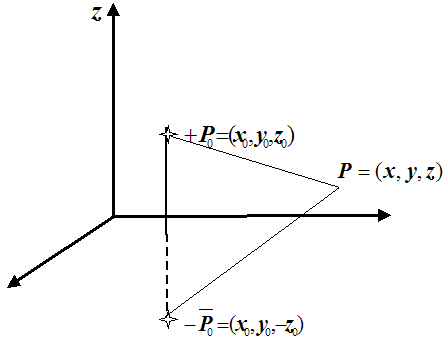
\includegraphics[]{img/20-1.png}
\end{figure}

Користуючись принципом суперпозиції електростатичних полів, легко зрозуміти, що компенсація потенціалу заряду в точці $P_0$ відбудеться у випадку, коли компенсуючий заряд розташувати дзеркально існуючому відносно площини $z = 0$, а величину заряду обрати одиничну зі знаком мінус. \medskip

В результаті отримаємо сумарний потенціал електростатичного поля:
\begin{equation}
	\begin{aligned}
		\Pi(P) &= \frac{1}{4 \pi |P - P_0|} - \frac{1}{4 \pi |P - \overline{P_0}|} = \\
		& = \frac{1}{4 \pi \sqrt{(x - x_0)^2 + (y - y_0)^2 + (z - z_0)^2}} - \\
		& \quad - \frac{1}{4 \pi \sqrt{(x - x_0)^2 + (y - y_0)^2 + (z + z_0)^2}}.
	\end{aligned}
\end{equation}

Легко перевірити, що 
\begin{equation}
	\left. \Pi(P) \right|_{P \in S} = 0.
\end{equation}

Таким чином побудована функція представляє собою функцію Гріна першої граничної задачі (Діріхле) оператора Лапласа для півпростору:
\begin{equation}
	\begin{aligned}
		G_1(P, P_0) &= \dfrac{1}{4 \pi \sqrt{(x - x_0)^2 + (y - y_0)^2 + (z - z_0)^2}} - \\
		& \quad - \dfrac{1}{4 \pi \sqrt{(x - x_0)^2 + (y - y_0)^2 + (z + z_0)^2}}.
	\end{aligned}
\end{equation}

Для знаходження розв'язку задачі Діріхле скористаємося формулою інтегрального представлення:
\begin{equation}
	U(P_0) = \Iiint_\Omega G_1(P, P_0) F(P) \diff P - \Iint_S \frac{\partial G_1(P, P_0)}{\partial n_P} f(P) \diff S_P.
\end{equation}

Обчислимо
\begin{equation}
	\begin{aligned}
		\left. \frac{\partial G_1(P, P_0)}{\partial n_P} \right|_{P \in S} &= - \frac{\partial}{\partial z} \left( \frac{1}{4 \pi \sqrt{(x - x_0)^2 + (y - y_0)^2 + (z - z_0)^2}} \right.- \\
		& \quad - \left. \frac{1}{4 \pi \sqrt{(x - x_0)^2 + (y - y_0)^2 + (z + z_0)^2}} \right) = \\
		& = - \left( \frac{z - z_0}{4 \pi ((x - x_0)^2 + (y - y_0)^2 + (z - z_0)^2)^{3/2}} \right. - \\
		& \quad - \left. \left. \frac{z - z_0}{4 \pi ((x - x_0)^2 + (y - y_0)^2 + (z + z_0)^2)^{3/2}} \right) \right|_{z = 0} = \\
		& = \frac{-z_0}{2 \pi (x - x_0)^2 + (y - y_0)^2 + z_0^2)^{3 / 2}}.
	\end{aligned}
\end{equation}

Таким чином, використовуючи формулу \eqref{eq:4.3.46} інтегрального представлення розв'язку першої граничної задачі, можемо записати розв'язок задачі Діріхле для рівняння Пуассона:
\begin{equation}
	\begin{aligned}
		U(x_0, y_0, z_0) &= \frac{1}{4 \pi} \Int_0^\infty \Iint_{\RR^2} \left( \frac{1}{\sqrt{(x - x_0)^2 + (y - y_0)^2 + (z - z_0)^2}} \right. - \\
		& \quad - \left. \frac{1}{\sqrt{(x - x_0)^2 + (y - y_0)^2 + (z + z_0)^2}} \right) F(x, y, z) \diff x \diff y \diff z + \\
		& \quad + \frac{z_0}{2 \pi} \Int_{-\infty}^\infty \Int_{-\infty}^\infty \frac{f(x, y) \diff x \diff y}{((x - x_0)^2 + (y - y_0)^2 + z_0^2)^{3/2}}
	\end{aligned}
\end{equation}

\subsubsection{Задача Неймана для півпростору}

Будемо розглядати граничну задачу:
\begin{system}
	& \Delta U(P) = - F(P), \quad P \in \Omega = \{(x, y, z): z > 0, x, y \in \RR\}, \\
	& - \left. \frac{\partial U(P)}{\partial z} \right|_{P \in S} = f(P), \quad S = \{(x, y, z): z = 0, x, y \in \RR\}.
\end{system}

Для знаходження розв'язку цієї задачі побудуємо функцію Гріна другої граничної задачі оператора Лапласа для півпростору. \medskip

Для випадку умови другого роду тобто коли на площині $z = 0$ виконується умова
\begin{equation}
	\left. \frac{\partial G_2(P, P_0)}{\partial n_P} \right|_{P \in S} = 0,
\end{equation}
її можна інтерпретувати як рівність нулю потоку електростатичного поля крізь площину $z = 0$. \medskip

Це означає, що поле внутрішнього одиничного заряду треба компенсувати полем зовнішніх зарядів. Це можна зробити, якщо дзеркально одиничному позитивному заряду в точці $P_0$ розташувати заряд додатного знаку в симетричній точці $\overline{P_0}$:
\begin{figure}[H]
	\centering
	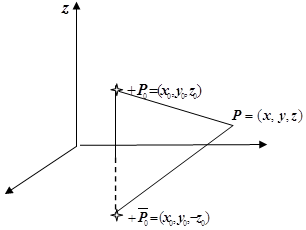
\includegraphics[]{img/20-2.png}
\end{figure}

Таким чином сумарний потенціал двох зарядів, а значить і функцію Гріна можна записати у вигляді:
\begin{equation}
	\begin{aligned}
		\Pi(P) &= \frac{1}{4 \pi |P - P_0|} + \frac{1}{4 \pi |P - \overline{P_0}|} = \\
		& = \frac{1}{4 \pi \sqrt{(x - x_0)^2 + (y - y_0)^2 + (z - z_0)^2}} + \\
		& \quad + \frac{1}{4 \pi \sqrt{(x - x_0)^2 + (y - y_0)^2 + (z + z_0)^2}} = G_2(P, P_0).
	\end{aligned}
\end{equation}

Перевіримо, що побудована функція Гріна задовольняє граничній умові:
\begin{equation}
	\begin{aligned}
		\left. \frac{\partial G_2(P, P_0)}{\partial n_P} \right|_{P \in S} &= - \frac{\partial}{\partial z} \frac{1}{4 \pi} \left( \frac{1}{\sqrt{(x - x_0)^2 + (y - y_0)^2 + (z - z_0)^2}} \right. + \\
		& \quad + \left. \left. \frac{1}{\sqrt{(x - x_0)^2 + (y - y_0)^2 + (z + z_0)^2}} \right) \right|_{z = 0} = \\
		& = \frac{1}{4 \pi} \left( \frac{z - z_0}{((x - x_0)^2 + (y - y_0)^2 + (z - z_0)^2)^{3/2}} \right. + \\
		& \quad + \left. \left. \frac{z + z_0}{((x - x_0)^2 + (y - y_0)^2 + (z + z_0)^2)^{3/2}} \right) \right|_{z = 0} = 0.
	\end{aligned}
\end{equation}

Враховуючи формулу \eqref{eq:4.3.47} інтегрального представлення розв'язку другої граничної задачі, отримаємо формулу для розв'язку задачі Неймана рівняння Пуассона в півпросторі:
\begin{equation}
	\begin{aligned}
		U(x_0, y_0, z_0) &= \frac{1}{4 \pi} \Int_0^\infty \Iint_{\RR^2} \left( \frac{1}{\sqrt{(x - x_0)^2 + (y - y_0)^2 + (z - z_0)^2}} \right. + \\
		& \quad + \left. \frac{1}{\sqrt{(x - x_0)^2 + (y - y_0)^2 + (z + z_0)^2}} \right) F(x, y, z) \diff x \diff y \diff z + \\
		& \quad + \frac{1}{2 \pi} \Int_{-\infty}^\infty \Int_{-\infty}^\infty \frac{f(x, y) \diff x \diff y}{((x - x_0)^2 + (y - y_0)^2 + z_0^2)^{3/2}}.
	\end{aligned}
\end{equation}

\end{document}